\section{Github}
- Link for every exercises in Lab 3: \href{https://github.com/Lmonk555/lab03_micro_process_control.git}{Link}

- Link for the testing video: \href{https://drive.google.com/file/d/1MUBsJ7rMVX56908bq_3bAQ5zY5j9nRom/view?usp=sharing}{Link}


\section{Problems Encountered}
- The PDF file didn't mention \texttt{HAL\_TIM\_Base\_Start\_IT(\&htim2);} in \texttt{main.c}. Remember to initialize it.\\

- In the lab session, we encounter lag when simulating on Proteus8. If you see the same problem, we recommend to change inside tab \texttt{System   ->  Set Animation Options}:
\begin{itemize}
    \item Frames per Second: 20 (by default)    ->  10
    \item Timestep per Frame: 50m (default)     ->  100m
\end{itemize}





\section{Exercise and Report}





\subsection{Specifications}
You are required to build an application of a traffic light in a cross road which includes some features as described below:
\begin{itemize}
    \item The application has 12 LEDs including 4 red LEDs, 4 amber LEDs, 4 green LEDs.
    \item The application has 4 seven segment LEDs to display time with 2 for each road. The 2 seven segment LEDs will show time for each color LED corresponding to each road.
    \item The application has three buttons which are used
    \subitem - to select modes, 
    \subitem - to modify the time for each color led on the fly, and 
    \subitem - to set the chosen value. 
    \item The application has at least 4 modes which is controlled by the first button. Mode 1 is a normal mode, while modes 2 3 4 are  modification modes. You can press the first button to change the mode. Modes will change from 1 to 4 and back to 1 again. 
    
    \textbf{Mode 1 - Normal mode}: 
    \subitem - The traffic light application is running normally.   
    
    \textbf{Mode 2 - Modify time duration for the red LEDs}: This mode allows you to change the time duration of the red LED in the main road. The expected behaviours of this mode include:  
    \subitem - All single red LEDs are blinking in 2 Hz. 
    \subitem - Use two seven-segment LEDs to display the value.
    \subitem - Use the other two seven-segment LEDs to display the mode.
    \subitem - The second button is used to increase the time duration value for the red LEDs. 
    \subitem - The value of time duration is in a range of 1 - 99. 
    \subitem - The third button is used to set the value.
    
    
    \textbf{Mode 3 - Modify time duration for the amber LEDs}: Similar for the red LEDs described above with the amber LEDs.
    
    
    \textbf{Mode 4 - Modify time duration for the green LEDs}: Similar for the red LEDs described above with the green LEDs.
\end{itemize}










\subsection{Exercise 1: Sketch an FSM}
Your task in this exercise is to sketch an FSM that describes your idea of how to solve the problem.

Please add your report here.\\

- In this exercise, we will notate:
\begin{itemize}
    \item BTN1: button 1 (same for the two others)
    \item R1/R2: Road 1/Road 2
\end{itemize}


\begin{figure}[H]
\centering
\begin{tikzpicture}[->, >=Stealth, node distance=4cm, auto,
  every state/.style={align=center, minimum size=2cm, font=\small}]
  \node[state, initial] (m1) {MODE 1\\Normal};
  \node[state, right of=m1] (m2) {MODE 2\\Set RED};
  \node[state, right of=m2] (m3) {MODE 3\\Set AMBER};
  \node[state, right of=m3] (m4) {MODE 4\\Set GREEN};
  \path (m1) edge node {BTN1} (m2)
        (m2) edge node {BTN1} (m3)
        (m3) edge node {BTN1} (m4)
        (m4) edge[bend left=35] node {BTN1} (m1);
\end{tikzpicture}
\caption{Mode FSM for Button 1}
\end{figure}


\begin{figure}[H]
\centering
\begin{tikzpicture}[->, >=Stealth, node distance=7.5cm, auto,
  every state/.style={align=center, minimum size=2.2cm, font=\small}]
  \node[state, initial] (s0) {R1: RED\\R2: GREEN};
  \node[state, right of=s0] (s1) {R1: RED\\R2: AMBER};
  \node[state, below of=s1, node distance=4cm] (s2) {R1: GREEN\\R2: RED};
  \node[state, left of=s2] (s3) {R1: AMBER\\R2: RED};
  \path (s0) edge node {R2\_Green ends} (s1)
        (s1) edge node {R2\_Amber ends} (s2)
        (s2) edge node {R1\_Green ends} (s3)
        (s3) edge node {R1\_Amber ends} (s0);
\end{tikzpicture}
\caption{Traffic light FSM in Mode 1}
\end{figure}


\begin{figure}[H]
\centering
\begin{tikzpicture}[->, >=Stealth, node distance=6cm, auto,
  every state/.style={align=center, minimum size=2cm, font=\small}]
  \node[state, initial] (b0) {RELEASED};
  \node[state, right of=b0] (b1) {PRESSED};
  \node[state, right of=b1] (b2) {PRESSED\\$>$1 s};
  \path (b0) edge[bend left] node {pressed / do action} (b1)
        (b1) edge[bend left] node {released} (b0)
        (b1) edge node {Hold for at least 1s} (b2)
        (b2) edge[bend left=50] node[swap] {released} (b0)
        (b2) edge[loop above] node {Repeat for every 500ms} (b2);
\end{tikzpicture}
\caption{Button FSM for mechanic in general}
\end{figure}










\subsection{Exercise 2: Proteus Schematic}
Your task in this exercise is to draw a Proteus schematic for the problem above. 

Please add your report here.


\textbf{\textit{Note:}} we will use this schematic for this whole lab session.


\begin{figure}[H]
    \centering
    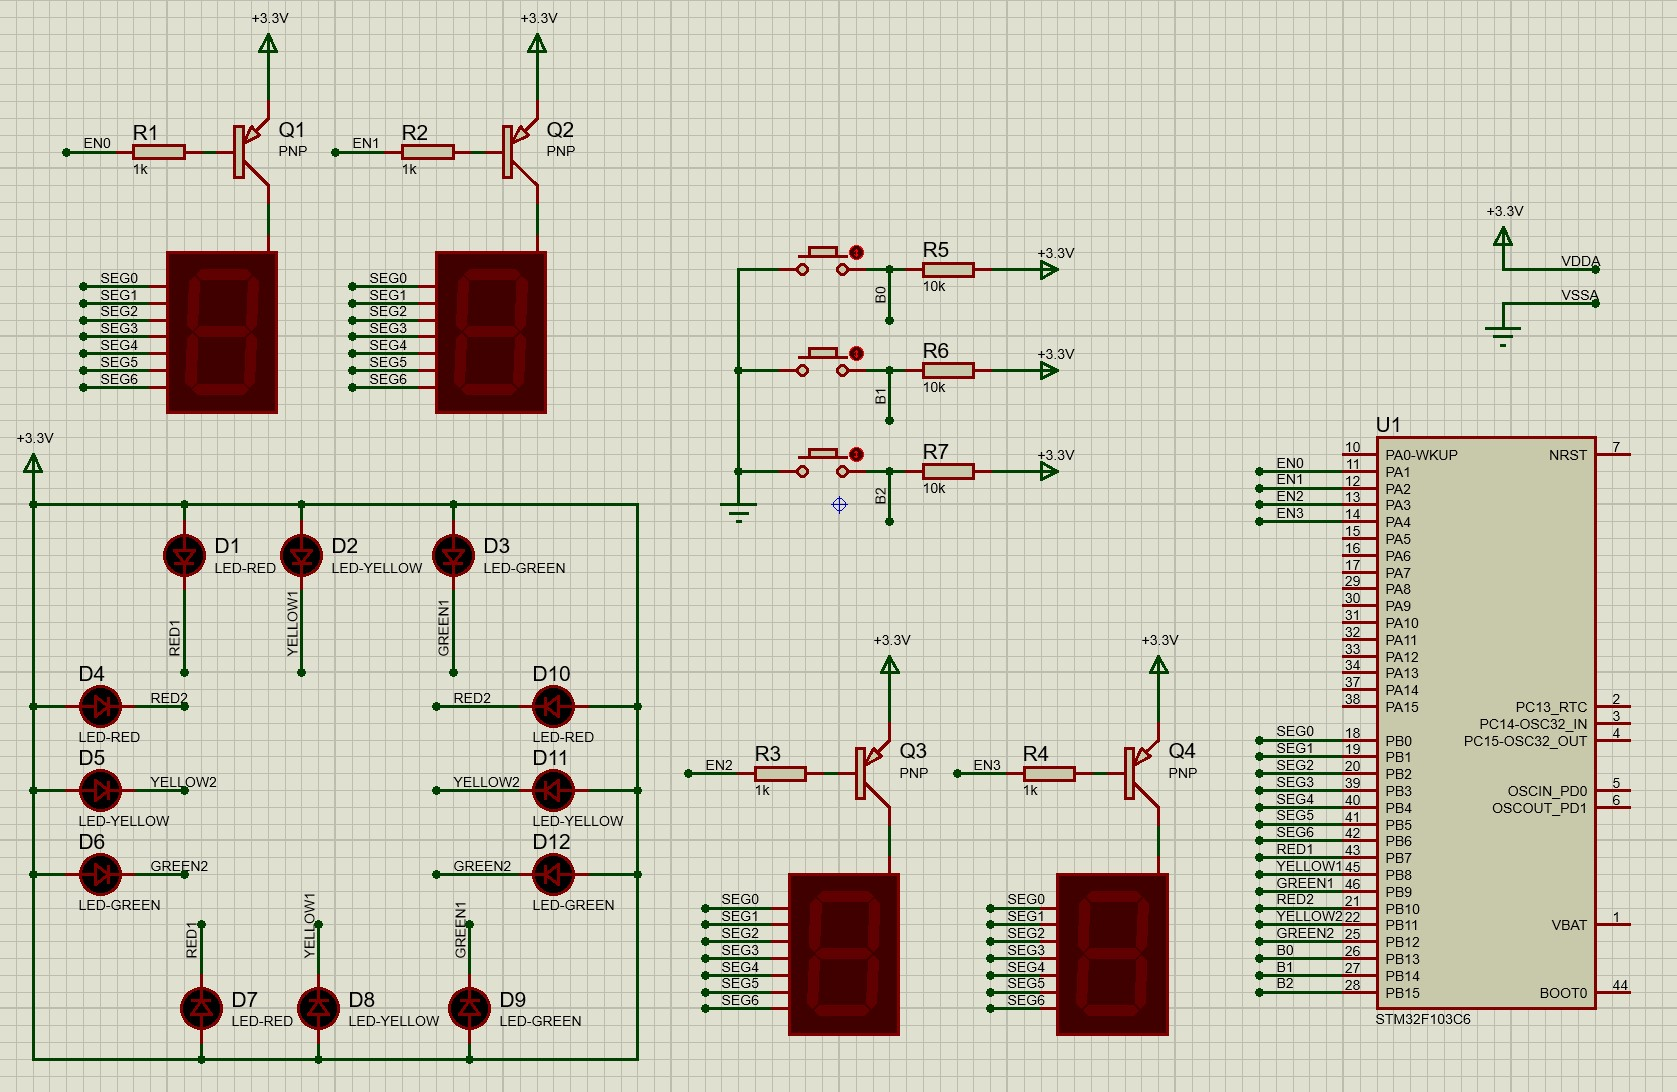
\includegraphics[width=0.8\linewidth]{pictures/schematic.jpg}
    \caption{{\textit{Proteus schematic for a formal 4-way traffic}}}
\end{figure}











\subsection{Exercise 3: Create STM32 Project}
Your task in this exercise is to create a project that has pin corresponding to the Proteus schematic that you draw in previous section. You need to set up your timer interrupt is about 10ms.

Please add your report here.\\

- We will initialize the necessay codes in the Exercise 4, other settings for the 10ms timer interrupt stay the same as the 2nd Lab session:
\begin{itemize}
    \item HCLK = 8 MHz
    \item Prescaler = 7999
    \item Counter Period = 9
\end{itemize}

\begin{figure}[H]
    \centering
    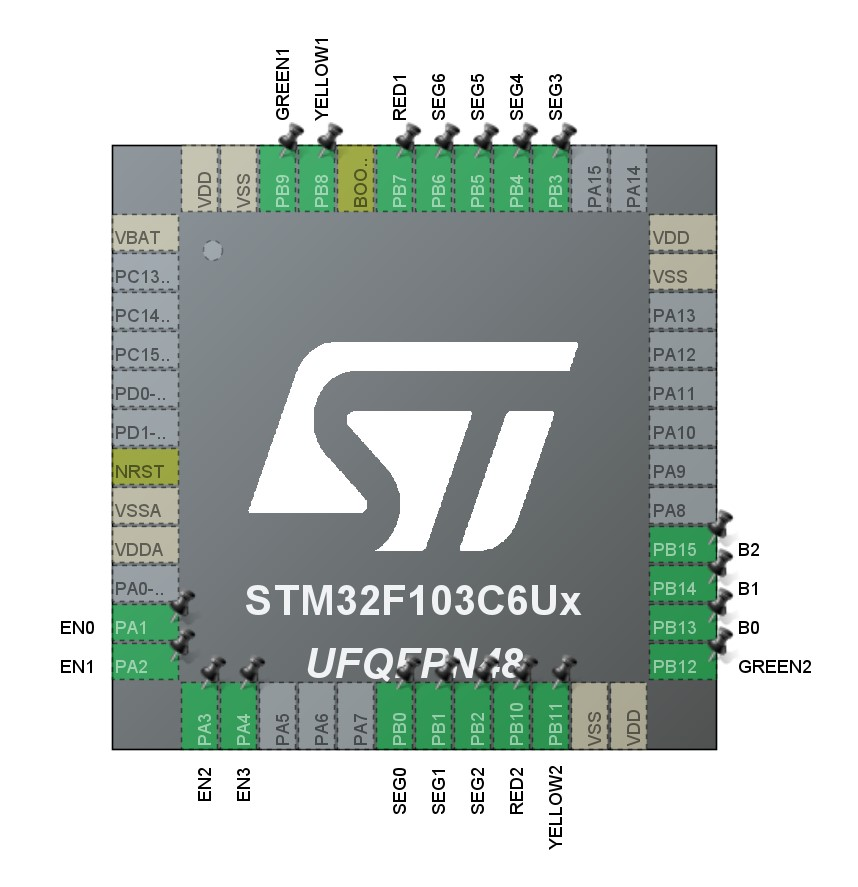
\includegraphics[width=0.8\linewidth]{pictures/stm32.jpg}
    \caption{{\textit{STM32CubeIDE schematic for a formal 4-way traffic}}}
\end{figure}










\subsection{Exercise 4: Modify Timer Parameters}
Your task in this exercise is to modify the timer settings so that when we want to change the time duration of the timer interrupt, we change it the least and it will not affect the overall system. For example, the current system we have implemented is that it can blink an LED in 2 Hz, with the timer interrupt duration is 10ms. However, when we want to change the timer interrupt duration to 1ms or 100ms, it will not affect the 2Hz blinking LED. 

Please add your report here.\\

- To do the exercise, we will implement the two files \texttt{timer.h} and \texttt{timer.c}.\\

\begin{lstlisting}[language=c,caption={Initial implementation for timer.h}]
#ifndef INC_TIMER_H_
#define INC_TIMER_H_

#include "main.h"

// Match the TIM2 interrupt period (in ms)
#define TIMER_CYCLE		1

// Timer indexes
#define TIMER_TRAFFIC	0	// 1 s tick for countdown
#define TIMER_BLINK		1	// 250 ms toggle -> 2 Hz blink
#define TIMER_SCAN		2	// 7-seg digit scanning
#define TIMER_AUTOINC	3	// BTN2 auto-repeat (500 ms)
#define MAX_TIMERS		4

void setTimer(int index, int duration_ms);
int  isTimerExpired(int index);
void timerRun(void);
void HAL_TIM_PeriodElapsedCallback(TIM_HandleTypeDef *htim);

#endif /* INC_TIMER_H_ */
\end{lstlisting}

% ==========================================================================================

\vspace{1em}
\begin{lstlisting}[language=c,caption={Add-on for timer.c}]
#include "timer.h"
#include "input_reading.h"

static int timerCounter[MAX_TIMERS];
static int timerFlag[MAX_TIMERS];

void setTimer(int index, int duration_ms)
{
    if (index < 0 || index >= MAX_TIMERS)	// Safety check
    	return;
    timerCounter[index] = duration_ms / TIMER_CYCLE;


    if (timerCounter[index] < 1)			// Safety check
    	timerCounter[index] = 1;			// in case of [duration_ms] too low, e.g. 5/10 = 0, we set a minimum = 1
    timerFlag[index] = 0;
}


int isTimerExpired(int index)
{
    if (index < 0 || index >= MAX_TIMERS) return 0;
    if (timerFlag[index])
    {
        timerFlag[index] = 0;				// clear on read: one event per expiry
        return 1;
    }
    return 0;
}


void timerRun(void)
{
    for (int i = 0; i < MAX_TIMERS; i++)
    {
        if (timerCounter[i] > 0)
        {
            timerCounter[i]--;
            if (timerCounter[i] == 0) timerFlag[i] = 1;
        }
    }
}


void HAL_TIM_PeriodElapsedCallback(TIM_HandleTypeDef *htim)
{
    if (htim->Instance == TIM2)
    {
        button_reading();
        timerRun();
    }
}

\end{lstlisting}

% ==========================================================================================

\vspace{1em}
- For confirmation when modifying Timer, we can use this example code below and change the relevant parameters (remember to update the \#include in \texttt{main.c} as it resets whenever you make changes in file \texttt{.ioc}).\\

- The code can be used for both cases.\\

\begin{table}[H]
    \centering
    \caption{Configuration for different Timer Interrupt}
    \label{tab:timer_config}
    \begin{tabular}{|c|c|c|c|}
        \hline
        \textbf{Timer Interrupt} & \textbf{Prescaler} & \textbf{Counter Period} & \textbf{TIMER\_CYCLE} \\
        \hline
        1 ms & 799 & 9 & 1 \\
        \hline
        10 ms & 7999 & 9 & 10 \\
        \hline
    \end{tabular}
\end{table}

\vspace{1em}
\begin{lstlisting}[language=c,caption={Temporary code for Exercise 4 test}]
/* Includes ------------------------------------------------------------------*/
#include "main.h"
#include "timer.h"


int main(void)
{
    MX_TIM2_Init();
    MX_GPIO_Init();

    /* USER CODE BEGIN 2 */
    HAL_TIM_Base_Start_IT(&htim2);
    setTimer(TIMER_BLINK, 250);
    /* USER CODE END 2 */

    while (1)
    {
        if (isTimerExpired(TIMER_BLINK))    // temporary test
        {
            setTimer(TIMER_BLINK, 250);
            HAL_GPIO_TogglePin(RED1_GPIO_Port, RED1_Pin);
        }
    }
}
\end{lstlisting}












\subsection{Exercise 5: Adding code for button debouncing}
Following the example of button reading and debouncing in the previous section, your tasks in this exercise are:
\begin{itemize}
    \item To add new files for input reading and output display,
    \item To add code for button debouncing,
    \item To add code for increasing mode when the first button is pressed. 
\end{itemize}

Please add your report here.\\

- For Exercise 5, we will adjust these files:
\begin{itemize}
    \item \texttt{input\_processing.h}
    \item \texttt{input\_reading.c}: add buttons ports and pins to read
    \item \texttt{input\_processing.c}: process the input button and return mode
    \item \texttt{led\_display.h}
    \item \texttt{led\_display.c}: display the 7-segment LED base on the mode
    \item \texttt{main.c}: change the testing codes to recent exercise
\end{itemize}

\vspace{1em}
- We also optimize some codes from the initial initialization but not changing its algorithm. Thus, we will present only what are added to the files.\\
- The test is expected to change modes by pressing button B0 and display the mode on the 7-segment LED EN0.

\begin{lstlisting}[language=c,caption={input\_reading.c}]
//we aim to work with more than one buttons
#define NO_OF_BUTTONS			3

//timer interrupt duration is 10ms, so to pass 1 second,
//we need to jump to the interrupt service routine 100 time
#define DURATION_FOR_AUTO_INCREASING	(1000 / TIMER_CYCLE)
#define BUTTON_IS_PRESSED				GPIO_PIN_RESET
#define BUTTON_IS_RELEASED				GPIO_PIN_SET

//the buffer that the final result is stored after debouncing
static GPIO_PinState buttonBuffer[NO_OF_BUTTONS]			= { GPIO_PIN_SET, GPIO_PIN_SET, GPIO_PIN_SET };;

//we define two buffers for debouncing
static GPIO_PinState debounceButtonBuffer1[NO_OF_BUTTONS]	= { GPIO_PIN_SET, GPIO_PIN_SET, GPIO_PIN_SET };;
static GPIO_PinState debounceButtonBuffer2[NO_OF_BUTTONS]	= { GPIO_PIN_SET, GPIO_PIN_SET, GPIO_PIN_SET };;

//we define a flag for a button pressed more than 1 second.
static uint8_t flagForButtonPress1s[NO_OF_BUTTONS];

//we define a counter for automatically increasing the value
//after the button is pressed more than 1 second.
static uint16_t counterForButtonPress1s[NO_OF_BUTTONS];

// From ex05
static GPIO_TypeDef *const	btnPort[NO_OF_BUTTONS]	= { B0_GPIO_Port, B1_GPIO_Port, B2_GPIO_Port };
static const uint16_t		btnPin[NO_OF_BUTTONS]	= { B0_Pin, B1_Pin, B2_Pin };


void button_reading(void)
{
    for(char i = 0; i < NO_OF_BUTTONS; i++)
    {
        debounceButtonBuffer2[i] = debounceButtonBuffer1[i];
        debounceButtonBuffer1[i] = HAL_GPIO_ReadPin(btnPort[i], btnPin[i]);

        if(debounceButtonBuffer1[i] == debounceButtonBuffer2[i])
        {
            buttonBuffer[i] = debounceButtonBuffer1[i];

            if(buttonBuffer[i] == BUTTON_IS_PRESSED)
            {
                //if a button is pressed, we start counting
                if(counterForButtonPress1s[i] < DURATION_FOR_AUTO_INCREASING)
                {
                    counterForButtonPress1s[i]++;
                }
                else
                {
                    //the flag is turned on when 1 second has passed
                    //since the button is pressed.
                    flagForButtonPress1s[i] = 1;
                }
            }
            else
            {
                counterForButtonPress1s[i] = 0;
                flagForButtonPress1s[i] = 0;
            }
        }
    }
}
\end{lstlisting}

% ==========================================================================================

\vspace{1em}
\begin{lstlisting}[language=c,caption={input\_processing.h}]
#ifndef INC_INPUT_PROCESSING_H_
#define INC_INPUT_PROCESSING_H_

#define MODE_NORMAL		1
#define MODE_RED		2
#define MODE_AMBER		3
#define MODE_GREEN		4
#define MODE_MAX		4

void fsm_for_input_processing(void);
int  get_mode(void);

#endif /* INC_INPUT_PROCESSING_H_ */
\end{lstlisting}

% ==========================================================================================

\vspace{1em}
\begin{lstlisting}[language=c,caption={input\_processing.c}]
// From ex05
static int mode = MODE_NORMAL;

int get_mode(void)
{
    return mode;
}

void fsm_for_input_processing(void)
{
    switch(buttonState)
    {
		case BUTTON_RELEASED:
			if(is_button_pressed(0))
			{
				buttonState = BUTTON_PRESSED;
				mode++;							// INCREASE VALUE OF PORT A BY ONE UNIT

				if (mode > MODE_MAX)
					mode = MODE_NORMAL;
			}
			break;


		case BUTTON_PRESSED:
			if(!is_button_pressed(0))
			{
				buttonState = BUTTON_RELEASED;
			}
			else if(is_button_pressed_1s(0))
			{
				buttonState = BUTTON_PRESSED_MORE_THAN_1_SECOND;
			}
			break;


		case BUTTON_PRESSED_MORE_THAN_1_SECOND:
			if(!is_button_pressed(0))
			{
				buttonState = BUTTON_RELEASED;
			}
			break;
    }
}
\end{lstlisting}

% ==========================================================================================

\vspace{1em}
\begin{lstlisting}[language=c,caption={led\_display.h}]
#ifndef INC_LED_DISPLAY_H_
#define INC_LED_DISPLAY_H_

void display7SEG(int num);

#endif /* INC_LED_DISPLAY_H_ */
\end{lstlisting}

% ==========================================================================================

\vspace{1em}
\begin{lstlisting}[language=c,caption={led\_display.c}]
#include "main.h"
#include "led_display.h"

typedef struct
{
    GPIO_TypeDef *port;
    uint16_t pin;
} SegPin;

SegPin segments[] =
{
    { SEG0_GPIO_Port, SEG0_Pin },
    { SEG1_GPIO_Port, SEG1_Pin },
    { SEG2_GPIO_Port, SEG2_Pin },
    { SEG3_GPIO_Port, SEG3_Pin },
    { SEG4_GPIO_Port, SEG4_Pin },
    { SEG5_GPIO_Port, SEG5_Pin },
    { SEG6_GPIO_Port, SEG6_Pin },
};

GPIO_PinState digitPatterns[10][7] =
{
    { RESET, RESET, RESET, RESET, RESET, RESET, SET   },	// 0
    { SET,   RESET, RESET, SET,   SET,   SET,   SET   },	// 1
    { RESET, RESET, SET,   RESET, RESET, SET,   RESET },	// 2
    { RESET, RESET, RESET, RESET, SET,   SET,   RESET },	// 3
    { SET,   RESET, RESET, SET,   SET,   RESET, RESET },	// 4
    { RESET, SET,   RESET, RESET, SET,   RESET, RESET },	// 5
    { RESET, SET,   RESET, RESET, RESET, RESET, RESET },	// 6
    { RESET, RESET, RESET, SET,   SET,   SET,   SET   },	// 7
    { RESET, RESET, RESET, RESET, RESET, RESET, RESET },	// 8
    { RESET, RESET, RESET, RESET, SET,   RESET, RESET },	// 9
};

void display7SEG(int num)
{
    if (num < 0 || num > 9) return;

	HAL_GPIO_WritePin(EN0_GPIO_Port, EN0_Pin, GPIO_PIN_SET);
	HAL_GPIO_WritePin(EN1_GPIO_Port, EN1_Pin, GPIO_PIN_SET);
	HAL_GPIO_WritePin(EN2_GPIO_Port, EN2_Pin, GPIO_PIN_SET);
	HAL_GPIO_WritePin(EN3_GPIO_Port, EN3_Pin, GPIO_PIN_SET);

    for (int i = 0; i < 7; i++)
        HAL_GPIO_WritePin(segments[i].port, segments[i].pin, digitPatterns[num][i]);
}
\end{lstlisting}

% ==========================================================================================

\vspace{1em}
\begin{lstlisting}[language=c,caption={main.c}]
#include "main.h"
#include "timer.h"
#include "input_processing.h"
#include "led_display.h"

MX_TIM2_Init();
MX_GPIO_Init();

/* USER CODE BEGIN 2 */
HAL_TIM_Base_Start_IT(&htim2);
static int lastMode = 0;
/* USER CODE END 2 */

while (1)
{
    //you only need to add the fsm function here
    fsm_for_input_processing();

    if (get_mode() != lastMode)
    {
        lastMode = get_mode();
        display7SEG(lastMode);
        HAL_GPIO_WritePin(EN0_GPIO_Port, EN0_Pin, GPIO_PIN_RESET);
    }
}
\end{lstlisting}






 



\subsection{Exercise 6: Adding code for displaying modes}
Your tasks in this exercise are:
\begin{itemize}
    \item To add code for display mode on seven-segment LEDs, and
    \item To add code for blinking LEDs depending on the mode that is selected. 
\end{itemize}

Please add your report here.\\

- For Exercise 6, we will adjust these files:
\begin{itemize}
    \item \texttt{input\_processing.h}
    \item \texttt{input\_processing.c}: add duration for the traffic lights and 7-segment LEDs
    \item \texttt{led\_display.h}
    \item \texttt{led\_display.c}: display the modes on EN0/EN1 and the duration of the conrresponding traffic lights on EN2/EN3, all through out the function \texttt{void fsm\_for\allowbreak{}\_output\allowbreak{}\_processing(void)}
    \item \texttt{main.c}: change the testing codes to recent exercise
\end{itemize}


\vspace{1em}
\begin{lstlisting}[language=c,caption={input\_processing.h}]
int get_duration(int index);            // 0 = red, 1 = amber, 2 = green
\end{lstlisting}

% ==========================================================================================

\vspace{1em}
\begin{lstlisting}[language=c,caption={input\_processing.c}]
int get_duration(int index)
{
    if (index < 0 || index > 2) return 0;
    return duration[index];
}
\end{lstlisting}

% ==========================================================================================

\vspace{1em}
\begin{lstlisting}[language=c,caption={led\_display.h}]
#ifndef INC_LED_DISPLAY_H_
#define INC_LED_DISPLAY_H_

void display7SEG(int num);

#endif /* INC_LED_DISPLAY_H_ */
\end{lstlisting}

% ==========================================================================================

\vspace{1em}
\begin{lstlisting}[language=c,caption={led\_display.h}]
void update_buffer(int mode, int value);	// fills the 4-digit buffer
void scan_leds(void);						// show the next digit
void leds_all_off(void);
void leds_toggle_color(int color);			// 0 = red, 1 = amber, 2 = green (both roads)

void output_init(void);
void fsm_for_output_processing(void);
\end{lstlisting}

% ==========================================================================================

\vspace{1em}
\begin{lstlisting}[language=c,caption={led\_display.c}]
void update_buffer(int mode, int value)
{
    led_buffer[0] = mode / 10;
    led_buffer[1] = mode % 10;
    led_buffer[2] = value / 10;
    led_buffer[3] = value % 10;
}

void scan_leds(void)
{
    display7SEG(led_buffer[index_led]);										// turns all EN off, writes the segments
    HAL_GPIO_WritePin(enPort[index_led], enPin[index_led], GPIO_PIN_RESET);	// enable one digit
    index_led = (index_led + 1) % 4;
}

void leds_all_off(void)														// active-low: SET = off
{
    for (int c = 0; c < 3; c++)
        for (int r = 0; r < 2; r++)
            HAL_GPIO_WritePin(ledPort[c][r], ledPin[c][r], GPIO_PIN_SET);
}

void leds_toggle_color(int color)
{
    if (color < 0 || color > 2) return;
    for (int r = 0; r < 2; r++)
        HAL_GPIO_TogglePin(ledPort[color][r], ledPin[color][r]);
}

void output_init(void)
{
    leds_all_off();
    setTimer(TIMER_SCAN, SCAN_PERIOD_MS);
}

void fsm_for_output_processing(void)
{
    static int lastMode = 0;
    int m = get_mode();

    if (m != lastMode)
    {
        lastMode = m;
        leds_all_off();
        setTimer(TIMER_BLINK, BLINK_PERIOD_MS);
    }


    if (m == MODE_NORMAL)
    	update_buffer(m, 0);
    else
    	update_buffer(m, get_duration(m - MODE_RED));


    if (isTimerExpired(TIMER_SCAN))
    {
        setTimer(TIMER_SCAN, SCAN_PERIOD_MS);
        scan_leds();
    }


    if (m != MODE_NORMAL && isTimerExpired(TIMER_BLINK))
    {
        setTimer(TIMER_BLINK, BLINK_PERIOD_MS);
        leds_toggle_color(m - MODE_RED);
    }
}
\end{lstlisting}

% ==========================================================================================

\vspace{1em}
\begin{lstlisting}[language=c,caption={main.c}]
HAL_TIM_Base_Start_IT(&htim2);
output_init();

while (1)
{
    //you only need to add the fsm function here
    fsm_for_input_processing();
    fsm_for_output_processing(); 
}
\end{lstlisting}










\subsection{Exercise 7: Adding code for increasing time duration value for the red LEDs}
Your tasks in this exercise are: 
\begin{itemize}
    \item to use the second button to increase the time duration value of  the red LEDs
    \item to use the third button to set the value for the red LEDs.
\end{itemize}
Please add your report here.\\


- For Exercise 7, we will adjust these files:
\begin{itemize}
    \item \texttt{input\_processing.h}
    \item \texttt{input\_processing.c}: add \texttt{static void button\_action(int index)} and update \texttt{fsm\_for\_input\_processing(void)}
    \item \texttt{led\_display.c}: slightly additional change
\end{itemize}


\vspace{1em}
\begin{lstlisting}[language=c,caption={input\_processing.h}]
int get_temp(void);				// value currently being edited
\end{lstlisting}

% ==========================================================================================


\vspace{1em}
\begin{lstlisting}[language=c,caption={input\_processing.c}]
int get_temp(void) { return tempValue; }

// What each button does when it is pressed (or auto-repeated)
static void button_action(int index)
{
    switch (index)
    {
		case 0:			// B0: next mode
			mode++;
			if (mode > MODE_MAX)
				mode = MODE_NORMAL;


			if (mode == MODE_NORMAL)
			    tempValue = 0;
			else
			    tempValue = duration[mode - MODE_RED];
			break;


		case 1:			// B1: increase temp value
			if (mode != MODE_NORMAL)
			{
				tempValue++;
				if (tempValue > 99)
					tempValue = 1;
			}
			break;


		case 2:			// B2: set (save) the value
			if (mode != MODE_NORMAL)
				duration[mode - MODE_RED] = tempValue;
			break;
    }
}

void fsm_for_input_processing(void)
{
    for (int i = 0; i < NUM_BUTTONS; i++)
    {
        switch (buttonState[i])
        {
			case BUTTON_RELEASED:
				if (is_button_pressed(i))
				{
					buttonState[i] = BUTTON_PRESSED;
					button_action(i);
				}
				break;


			case BUTTON_PRESSED:
				if (!is_button_pressed(i))
				{
					buttonState[i] = BUTTON_RELEASED;
				}
				else if (is_button_pressed_1s(i))
				{
					buttonState[i] = BUTTON_PRESSED_MORE_THAN_1_SECOND;

					if (i == 1)
						setTimer(TIMER_AUTOINC, AUTO_REPEAT_MS);
				}
				break;


			case BUTTON_PRESSED_MORE_THAN_1_SECOND:
				if (!is_button_pressed(i))
				{
					buttonState[i] = BUTTON_RELEASED;
				}
				else if (i == 1 && isTimerExpired(TIMER_AUTOINC))		// auto-repeat only for B1
				{
					setTimer(TIMER_AUTOINC, AUTO_REPEAT_MS);
					button_action(1);
				}
				break;
        }
    }
}

\end{lstlisting}

% ==========================================================================================

\vspace{1em}
\begin{lstlisting}[language=c,caption={led\_display.c}]
void fsm_for_output_processing(void)
{
    /*
    ...
    */

    if (m == MODE_NORMAL)
    	update_buffer(m, 0);
    else
    	update_buffer(m, get_temp());


    if (isTimerExpired(TIMER_SCAN))
    /*
    ...
    */
}
\end{lstlisting}










\subsection{Exercise 8: Adding code for increasing time duration value for the amber LEDs}

Your tasks in this exercise are: 
\begin{itemize}
    \item to use the second button to increase the time duration value of the amber LEDs
    \item to use the third button to set the value for the amber LEDs.
\end{itemize}
Please add your report here.\\

- Modifying the amber duration reuses the mechanism built in Exercise~7, so no new code is needed. The color being edited is not hard-coded: it is derived from the current mode as \texttt{mode - MODE\_RED}, which gives index 0 for red (Mode~2), 1 for amber (Mode~3) and 2 for green (Mode~4). The three saved durations are stored in a single array \texttt{duration[3]}, initialized to 5, 2 and 3 seconds for red, amber and green respectively.

- When the first button (B0) moves the system into Mode~3, a temporary value \texttt{tempValue} is loaded from the saved amber duration (\texttt{duration[1]}). The second button (B1) increases \texttt{tempValue} by one on each press and wraps from 99 back to 1, so the value always stays in the range 1--99. If B1 is held for more than one second, the button FSM enters the \texttt{BUTTON\_PRESSED\_MORE\_THAN\_1\_SECOND} state and the value increases automatically every 500~ms. The third button (B2) copies \texttt{tempValue} into \texttt{duration[1]}, which saves the new amber duration. If the user leaves the mode without pressing B2, the edit is discarded, because the next entry into the mode reloads \texttt{tempValue} from the saved value.

- For the display, the two seven-segment LEDs on EN0 and EN1 show the mode number (\texttt{03}) and the two LEDs on EN2 and EN3 show \texttt{tempValue}. The four digits are multiplexed by scanning one digit every 10~ms. While in this mode, only the amber LEDs of both roads blink at 2~Hz, using a software timer that toggles them every 250~ms; the other colors stay off.










\subsection{Exercise 9: Adding code for increasing time duration value for the green LEDs}

Your tasks in this exercise are: 
\begin{itemize}
    \item to use the second button to increase the  time duration value of the green LEDs
    \item to use the third button to set the value for the green LEDs.
\end{itemize}
Please add your report here.\\

- Modifying the green duration works exactly like the amber and red cases, since all three share the same code. In Mode~4 the index \texttt{mode - MODE\_RED} evaluates to 2, so the button actions operate on \texttt{duration[2]}, whose default value is 3 seconds.










\subsection{Exercise 10: To finish the project}
Your tasks in this exercise are:
\begin{itemize}
    \item To integrate all the previous tasks to one final project
    \item To create a video to show all features in the specification
    \item To add a report to describe your solution for each exercise.
    \item To submit your report and code on the BKeL
\end{itemize}

- For the final and complete project, we will adjust only one file \texttt{led\_display.c} in order to display the real traffic cycle. Moreover, we have to handle the wrong button inputs (e.g. set duration for RED - AMBER - GREEN to 7/7/7 seconds respectively).

- By initializing hard constraint:
\begin{lstlisting}[language=c]
int gap = R - G - A;      // how much longer the saved red is than green + amber
if (gap < 0) gap = 0;     // red can't be shorter than that, so no negative gap
int redTime = G + A + gap;
\end{lstlisting}
we can let the traffic lights run smoothly despite the wrong inputs.\\

- For the detail codes, please check over \texttt{STM32CubeIDE/lab\_03/Core/Src/led\_display.c}.
















































% I don't know what this shi
% sign: Lmonk


% \section{Problem 1}

% In this week lab, assume you have two button and 8 LEDs, you have to write a program that
% \begin{itemize}
%     \item Has a timer which has an interrupt in every 10 milliseconds.  
%     \item  Reads values of buttons 1 and 2 every 10 milliseconds. The read button function should be called inside the timer interrupt service routine.
%     \item Increases the value of LEDs connected to PORTA when the button 1 is pressed.
%     \item Increases the value of PORTA automatically in every 0.5 second, if the button 1 is pressed in more than 1 second.
%     \item Increases the value of PORTA automatically in every 0.1 second, if the button 1 is pressed in more than 3 seconds.
%     \item Decreases the value of PORTA when the button 2 is pressed
%     \item Decreases the value of PORTA automatically in every 0.5 second, if the button 2 is pressed in more than 1 second.
%     \item Decreases the value of PORTA automatically in every 0.1 second, if the button 2 is pressed in more than 3 seconds.
%     \item The above values such as 10 ms, 0.5 s, 0.1s, 1 s and 3 s are fixed values as an example. Your program, however, needs to provide an easy way to change those values. For example, you should use DEFINE to define those values.
%     \item If both buttons 1 and 2 are pressed, button 1 has a higher priority.
% \end{itemize}


% \section{Problem 2 - A digital clock}
%  You have to write a program that mimics a Casio digital watch. Assume you have 2 buttons and 6 seven-segment LED, a program should have
% \begin{itemize}
%     \item A normal clock that shows hours, minutes, and seconds on 6 seven-segment LEDs.
%     \item  A stopwatch that shows minutes, seconds and 1/100 second
%     \item We use button 1 to change modes of a digital watch. Every time button 1 is pressed, the watch will change to the next mode.
%     \item Mode 0: runs normal clock (default)
%     \item Mode 1: modifies hours. In this mode, the hour number is blinking, and button 2 is used for increasing the hour number.  If button 2 is kept pressed more than 1 second, the hour number will increase automatically, i.e., 5 times per second. Please note that the hour number should be returned to 0 when it reaches 23.
%     \item  Mode 2: modifies minutes. Similar to mode 1, the minute number is blinking and increases when button 2 is pressed.
%     \item Mode 3: modifies seconds. Similar to mode 1, the second number is blinking and increases when button 2 is pressed.
%     \item Mode 4: runs a stopwatch. Using button 2 to start and stop the watch.  
 
% \end{itemize}
%  Please note that while the stopwatch is running, the normal clock is still running in the background.


 

% \section{Instructions}

% Your task is to sketch an FSM that describes your idea of how to solve the above problems and  writes a firmware that runs on STM32.



 

% \section{Submission}

% You need to
% \begin{itemize}
%     \item Demonstrate your work in the lab class and then
%     \item  Submit your FSM sketches and source code to the BKeL.
% \end{itemize}
